\section{Examenes}

\subsection{Primer examencillo de la clase de practicas}
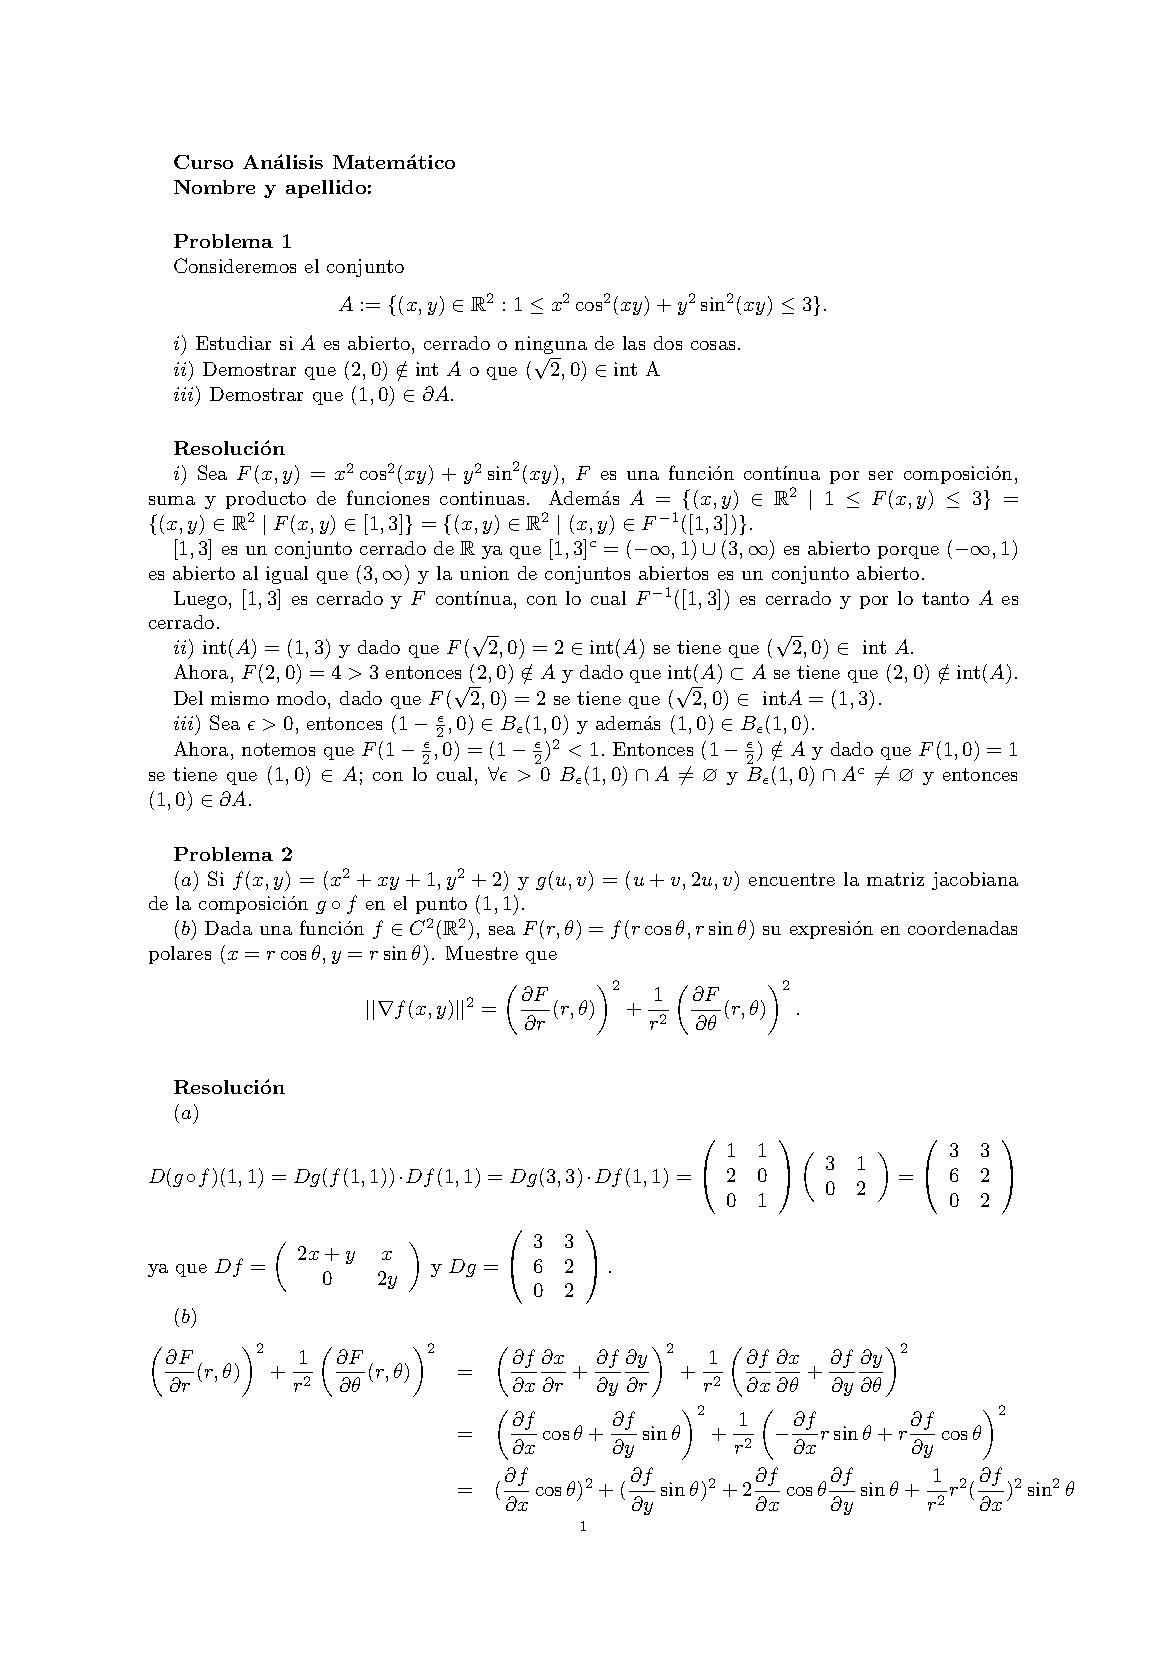
\includepdf[pages={1-last}]{Practicas/_primer_examencillo.pdf}
\subsection{Parcial 1}

\begin{problem}[1]

$\appl{d}{\real^2}{\real}$ homogenea\footnote{$(f(tx,ty) = t^mf(x,y)$} con $m>0$. F acotada superiormente sobre la circunferencia unidad.

a) Probar que $F$ es continua en $(0,0)$
b) Si $m=0$ ¿F continua en (0,0)?
\solution
\paragraph{Apartado a:}
\subparagraph{1)}
Vamos a ver que $F(0,0) = 0$.

$F(0,0) = F(t0,t0) = t^mF(0,0) \implies F(0,0) = 0$

\subparagraph{2)}
Aplicando la caracterización por sucesiones de la continuidad: $\{X_n\} \rightarrow 0 \implies F(X_n) \rightarrow 0$ si $F$ continua.

Sea $Z_n = \{(X_n,Y_n)\}, n\in \mathbb{N}$ una sucesión tal que $Z_n \rightarrow (0,0)$.

\begin{gather*}\abs{F_n} = \abs{F\left(\frac{Z_n}{\md{Z_n}}\md{Z_n}\right)} =
\md{X_n}^n \abs{F\left(\frac{Z_n}{\md{Z_n}}\right)} \implies \\
\exists M>0 \tlq \md{Z_n}^n \abs{F\left(\frac{Z_n}{\md{Z_n}}\right)} \leq \md{Z_n}^n M \rightarrow 0 = F(0,0)
\end{gather*}
\paragraph{Apartado b:}
Sí, $m=0 \implies F$ constante. Se puede demostrar pasando a coordenadas polares $x=rcos(t),y=rsen(t)$

\end{problem}

%\begin{problem}[2]
%\solution
%\end{problem}
\section{Examen Enero 2013}
\subsection{1:}

Sea $f\in C^2(\mathbb{R})$ tal que $f(2) = 0$, $f'(2)=1$. Consideramos la ecuación \\$$F(x,y,z) = x^2+y^2+z^2-f(2+Cz)=0$$

\paragraph{a)} Probar que existen un abierto $U\subset \mathbb{R}^2$ con $(0,0)\in U$, y un abierto $V\subset \mathbb{R}$ con $0\in V$, y una función $C^1$\\$$\phi: U \rightarrow V$$\\tal que $F(x, y, \phi (x, y)) = 0$ para todo $(x,y) \in U$\\

\textbf{Solución:}\\
$\frac{\delta F}{\delta z}(0,0,0) = 2z - f'(2+Cz)C (0,0,0) =-f'(2)C = -C \neq 0$
con lo cual si $c\neq 0$, por el teorema de la función implícita, existen entornos $U\subset \mathbb{R}^2$ y $V\subset{R}$ con $(0,0)\in U, 0\in V$ y una función $\appl{\phi}{U}{V}$ de clase $C^1$ con $\phi (0,0) = 0$ tal que $F(x,y,\phi (x,y)) = 0 \forall (x,y)\in U$

Falta comprobar el resto de hipótesis del teorema de la función implícita.

\paragraph{b)} Hallar las derivadas parciales de la función encontrada en el apartado anterior y demostrar que \\

$$y\frac{\delta \phi (x,y)}{\delta x} - x\frac{\delta \phi (x,y)}{\delta y} = 0$$

\textbf{Solución:}
Derivamos implícitamente respecto de x:\\
$$2\phi (x,y) \frac{\delta \phi (x,y)}{\delta x} - f'(2+C\phi (x,y))C\frac{\delta \phi (x,y)}{\delta x}=-2x$$\\
$$\hdots$$\\
$$\frac{\delta \phi (x,y)}{\delta x} = \frac{-2x}{2\phi (x,y) - Cf'(2+C\phi (x,y)}$$ si $2\phi (x,y) \neq Cf'(2+C\phi (x,y))$
\\Procediendo del mismo modo: \\
$$\frac{\delta \phi (x,y)}{\delta y} = \frac{-2y}{2\phi (x,y) - Cf'(2+C\phi (x,y)}$$ si $2\phi (x,y) \neq Cf'(2+C\phi (x,y))$\\
Multiplicando a ambos lados la derivada parcial con respecto a $x$ por $y$ y la derivada parcial con respecto a $y$ por $x$ llegamos a que\\ $$y\frac{\delta \phi (x,y)}{\delta x} = x\frac{\delta \phi (x,y)}{\delta y}$$, que era lo que queríamos demostrar.

\paragraph{c)} Estudiar si la función $\phi$ alcanza un extremo relativo en $(0,0)$, y determinar su tipo (en función de la constante C).

\textbf{Solución:}\\
$$x^2 + y^2 + (\phi (x,y))^2 -f(2+C\phi (x,y)) = 0$$\\
$$\frac{\delta \phi}{\delta x}(0,0) = \frac{0}{C} = 0$$
$$\frac{\delta \phi}{\delta y}(0,0) = \frac{0}{C} = 0$$
$\implies \phi$ tiene en $(0,0)$ un extremo relativo.\\

Procedemos a calcular su tipo:\\
$$\frac{\delta F}{\delta x}: 2x-2\phi (x,y)\frac{\delta \phi}{\delta x}-f'(2+C\phi (x, y))C\frac{\delta \phi}{\delta x} = 0$$\\
$$\frac{\delta ^2 F}{\delta x^2}(0,0): 2-2[(\frac{\delta \phi (x,y)}{\delta x})^2] - f''(2+C\phi (x,y))C^2(\frac{\delta \phi}{\delta x})^2$$

Lo siento chicos... no me ha dado tiempo a copiar, es mi primer día copiando cálculo. Pero el resultado es que el extremo es:

\begin{itemize}
\item Mínimo si $C>0$
\item Máximo si $C<0$
\item Nada si $C=0$ porque $2/C$ no estaría definido. 
\end{itemize}

No se hacer matrices, pero si os apetece completar el hessiano es $(2/C, 0)$ la primera fila, y $(0, 2/C)$ la segunda fila. Por tanto el determinante da $4/C^2 > 0$ y hay que analizar el término en la fila uno, columna uno de la matriz.

\section{Examen Junio 2013}
\subsection{1)} Sea $\appl{f}{\mathbb{R}^3}{\mathbb{R}}$. Se dice que f es homogénea de grado m si\\
$$f(\lambda x, \lambda y, \lambda z) = \lambda ^m f(x,y,z)$$ para todo $\lambda > 0$.

\paragraph{a)} Si f es diferenciable y homogénea de grado $m>0$ demostrar que:
$$<\nabla f(x,y,z), (x,y,z) > = mf(x,y,z)$$
\textbf{Solución:}\\
$$x\frac{\delta f}{\delta x}(x,y,z) + y\frac{\delta f}{\delta y}(x,y,z) + z\frac{\delta f}{\delta z}$$
derivamos respecto de $\lambda$

$$\frac{\delta f}{\delta \lambda}(\lambda x, \lambda y, \lambda z) = \underbrace{\frac{\delta}{\delta \lambda}(\lambda^mf(x,y,z))}_{m\lambda^{m-1}f(x,y,z)}$$

$$\frac{\delta f}{\delta \lambda x}\frac{\delta \lambda x}{\delta \lambda} + \frac{\delta f}{\delta \lambda y}\frac{\delta \lambda y}{\delta \lambda} + \frac{\delta f}{\delta \lambda z}\frac{\delta \lambda z}{\delta \lambda} = \frac{\delta f}{\delta \lambda x}x + \frac{\delta f}{\delta \lambda y}y + \frac{\delta f}{\delta \lambda z}z = m\lambda ^{m-1} f(x,y,z) $$

$$<\nabla f(\lambda x,\lambda y,\lambda z), (x,y,z) > = m\lambda^{m-1} f(x,y,z)\ \forall \lambda > 0$$

Si tomamos $\lambda = 1$ entonces $$<\nabla f(x,y,z), (x,y,z) > = mf(x,y,z)$$ que era lo que queríamos demostrar.\footnote{Este es el teorema de euler de las funciones homogéneas, y sí, te piden demostrarlo en un examen, extraordinrio}

\paragraph{b)} Supongamos $f$ continua sobre la esfera ${x^2+y^2+z^2=1}$. Supongamos que $f$ es homogénea de grado $m = 0$, y que $f(0,0,0) = 0$.

\begin{itemize}
\item Estudiar la continuidad de $f$ en el origen.
\item Estudiar la continuidad de $f$ en el resto de puntos del espacio.
\end{itemize}

\textbf{Solución:}\\
Considero $\lambda = \frac{1}{\norm{(x,y,z)}}$\footnote{Esto es una idea feliz.}\\
$$f(x,y,z) = f(\lambda x, \lambda y, \lambda z)$$
Si f es continua en $x_1$ lo va a ser en $x_2$ con $x_1 = \lambda x_2$ por se homogénea.\footnote{Es como tomar un punto $x_2$ en una esfera más pequeña de la esfera de radio uno, y si unimos ese punto con el $x_1$ que esta en la esfera de radio uno, por ser homogénea va a ser contínua en la recta que los une.}

Formalmente:
$$\forall \epsilon > 0, \exists \delta > 0 \tq si \norm{x-y} < \delta \implies \norm{f(x) - f(y)} < \epsilon$$

$$\norm{x - 0} < \delta \implies \abs{f(x,y,z) - \underbrace{f(0,0,0)}_{=0}} < \epsilon$$
$$\abs{f(x,y,z)} < \epsilon\ \forall \epsilon > 0$$
$$ f = 0$$
$$ \frac{x}{\norm{x}} - \frac{y}{\norm{y}} < \norm{x-y}$$


\subsection{Examencillo de clase de Pr\'acticas del d\'ia 29-noviembre}
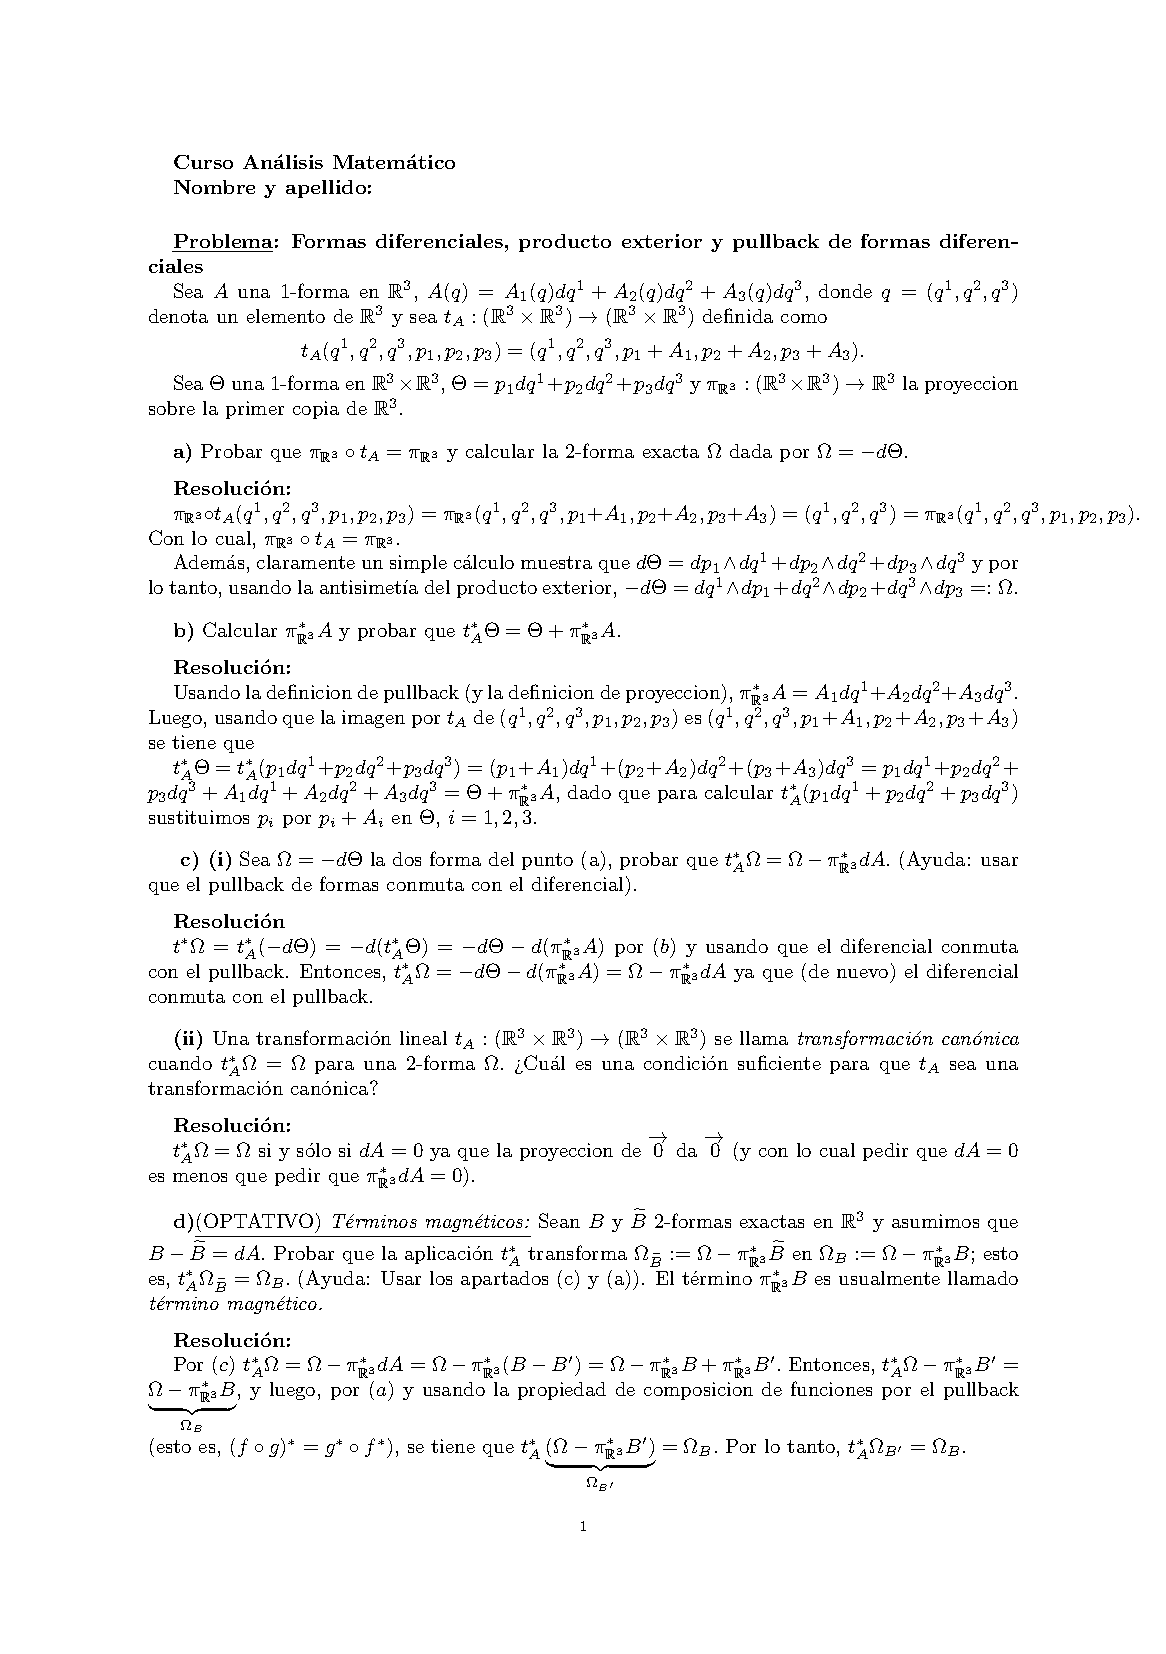
\includepdf{Practicas/_Problema_formas_diferenciales_Leo.pdf}